\documentclass{standalone}
\usepackage{tikz}
\usetikzlibrary{patterns, positioning}
\usepackage[sfdefault]{ClearSans} %% option 'sfdefault' activates Clear Sans as the default text font
\usepackage[T1]{fontenc}

\begin{document}
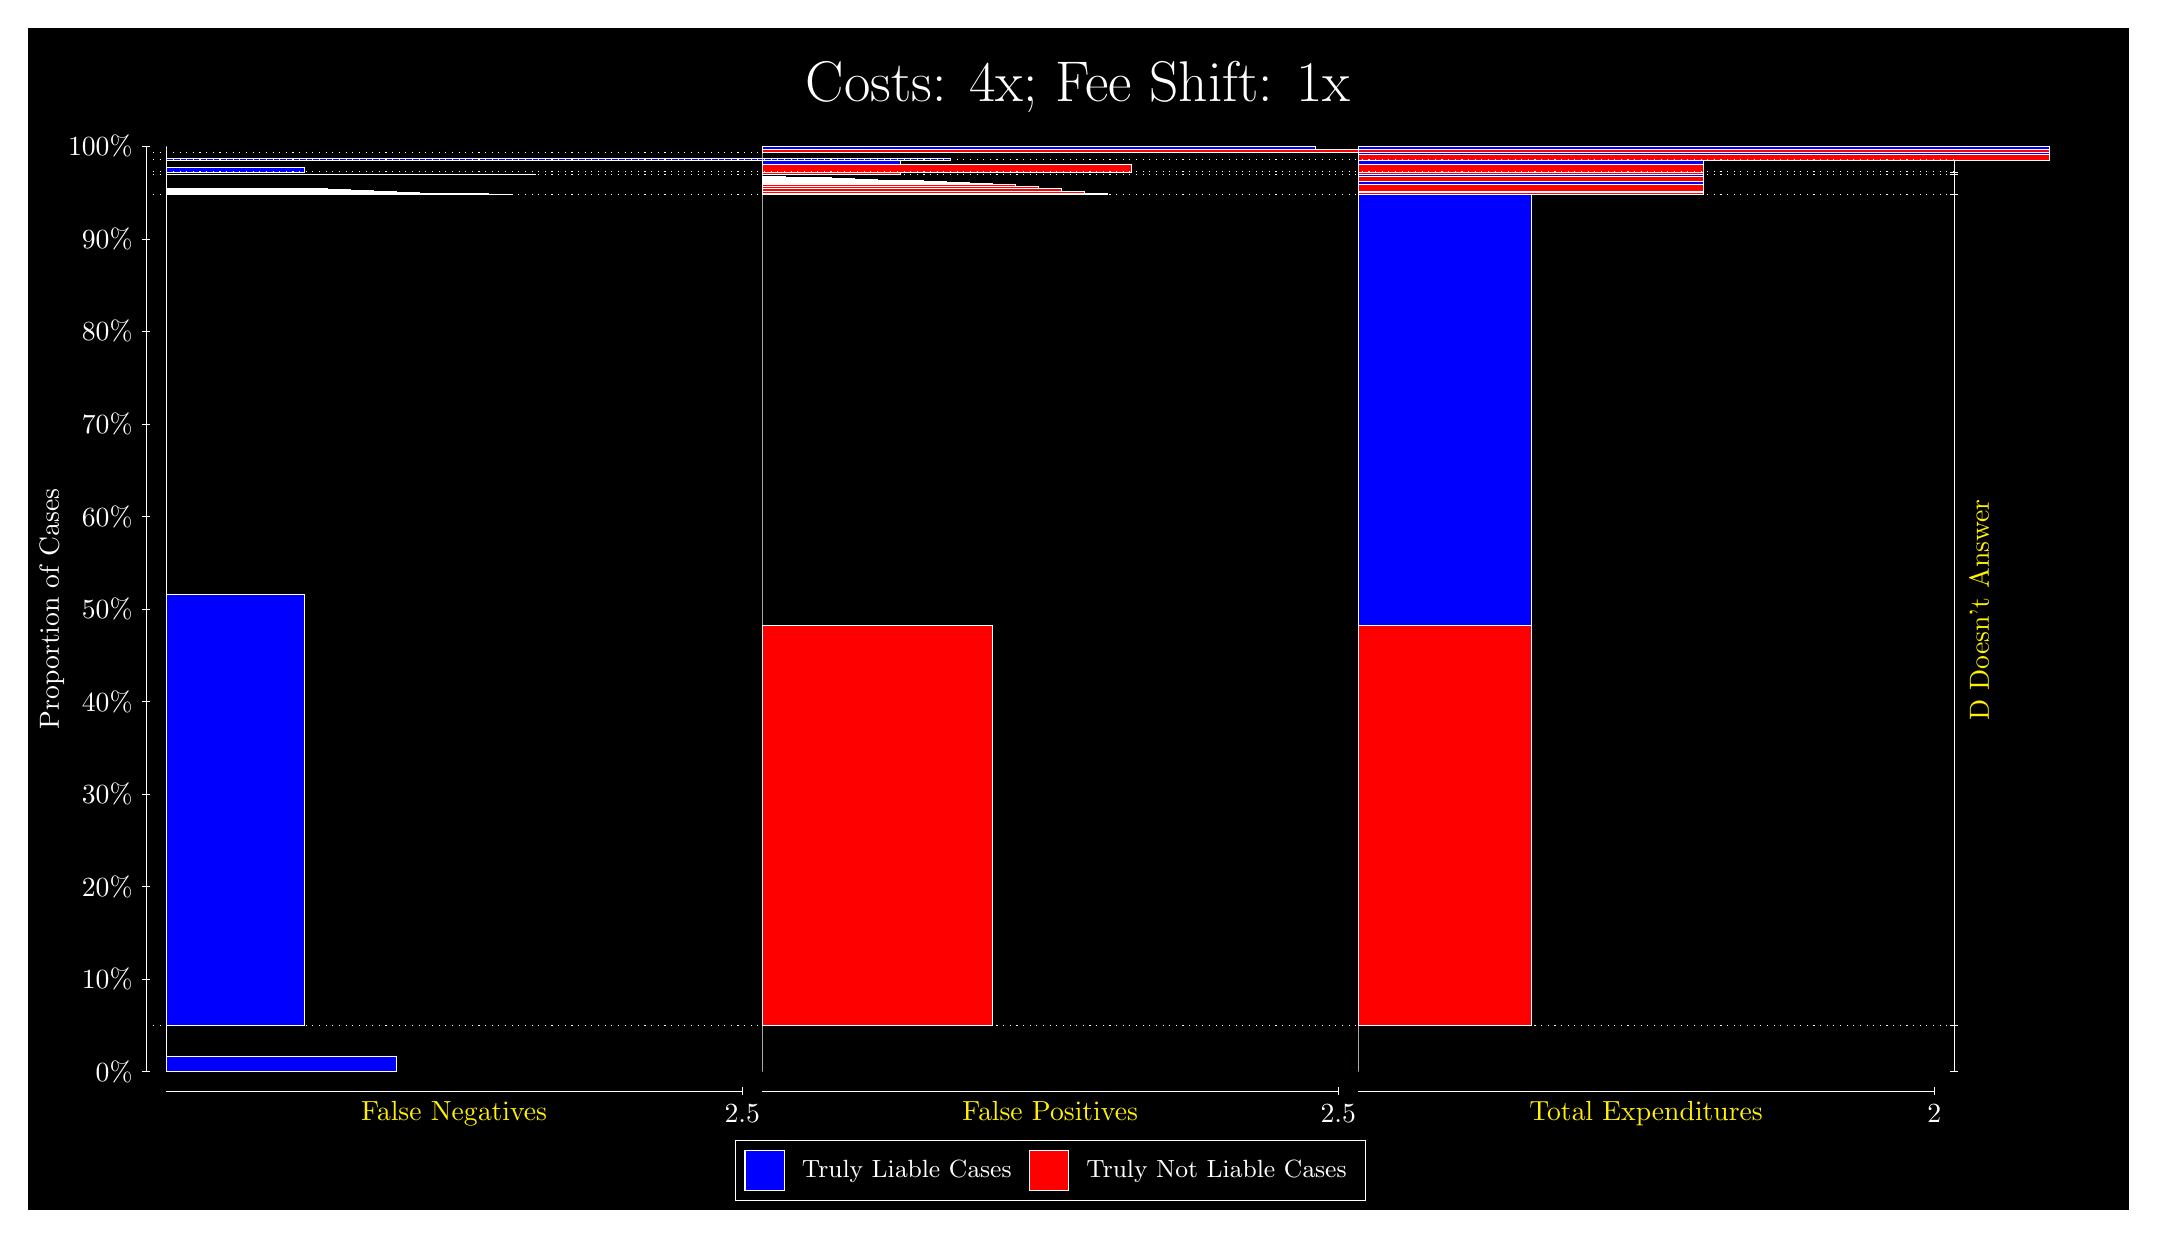
\begin{tikzpicture}
\draw[fill=black] (0,0) rectangle (26.667,15);
\draw[text=white] (0,13.5) rectangle (26.667,15) node[midway] {\huge Costs: 4x; Fee Shift: 1x};
\draw[white, very thin] (1.5,1.75) -- (1.5,13.5);
\node[rotate=90, text=white, anchor=center] at (0.3, 7.625) {Proportion of Cases};
\draw[white, very thin] (1.45,1.75) -- (1.55,1.75);
\node[text=white, anchor=east] at (1.45, 1.75) {0\%};
\draw[white, very thin] (1.45,2.925) -- (1.55,2.925);
\node[text=white, anchor=east] at (1.45, 2.925) {10\%};
\draw[white, very thin] (1.45,4.1) -- (1.55,4.1);
\node[text=white, anchor=east] at (1.45, 4.1) {20\%};
\draw[white, very thin] (1.45,5.275) -- (1.55,5.275);
\node[text=white, anchor=east] at (1.45, 5.275) {30\%};
\draw[white, very thin] (1.45,6.45) -- (1.55,6.45);
\node[text=white, anchor=east] at (1.45, 6.45) {40\%};
\draw[white, very thin] (1.45,7.625) -- (1.55,7.625);
\node[text=white, anchor=east] at (1.45, 7.625) {50\%};
\draw[white, very thin] (1.45,8.8) -- (1.55,8.8);
\node[text=white, anchor=east] at (1.45, 8.8) {60\%};
\draw[white, very thin] (1.45,9.975) -- (1.55,9.975);
\node[text=white, anchor=east] at (1.45, 9.975) {70\%};
\draw[white, very thin] (1.45,11.15) -- (1.55,11.15);
\node[text=white, anchor=east] at (1.45, 11.15) {80\%};
\draw[white, very thin] (1.45,12.325) -- (1.55,12.325);
\node[text=white, anchor=east] at (1.45, 12.325) {90\%};
\draw[white, very thin] (1.45,13.5) -- (1.55,13.5);
\node[text=white, anchor=east] at (1.45, 13.5) {100\%};

\draw[white, very thin] (24.457,1.75) -- (24.457,13.5);
\draw[white, very thin] (24.407,1.75) -- (24.507,1.75);
\node[anchor=west] at (24.407, 1.75) {};
\draw[white, very thin] (24.407,2.3311) -- (24.507,2.3311);
\node[anchor=west] at (24.407, 2.3311) {};
\draw[white, very thin] (24.407,12.889) -- (24.507,12.889);
\node[anchor=west] at (24.407, 12.889) {};
\draw[white, very thin] (24.407,13.143) -- (24.507,13.143);
\node[anchor=west] at (24.407, 13.143) {};
\draw[white, very thin] (24.407,13.175) -- (24.507,13.175);
\node[anchor=west] at (24.407, 13.175) {};
\draw[white, very thin] (24.407,13.327) -- (24.507,13.327);
\node[anchor=west] at (24.407, 13.327) {};
\draw[white, very thin] (24.407,13.425) -- (24.507,13.425);
\node[anchor=west] at (24.407, 13.425) {};
\draw[white, very thin] (24.407,13.5) -- (24.507,13.5);
\node[anchor=west] at (24.407, 13.5) {};

\draw[white, very thin, fill=blue] (1.75,1.75) rectangle (4.6775,1.9425);
\draw[white, very thin, fill=red] (1.75,1.9425) rectangle (1.75,2.3311);
\draw[white, very thin, fill=blue] (1.75,2.3311) rectangle (3.5065,7.8069);
\draw[white, very thin, fill=red] (1.75,7.8069) rectangle (1.75,12.889);
\draw[white, very thin, fill=blue] (1.75,12.889) rectangle (6.1413,12.896);
\draw[white, very thin, fill=blue] (1.75,12.896) rectangle (5.8486,12.899);
\draw[white, very thin, fill=blue] (1.75,12.899) rectangle (5.5558,12.905);
\draw[white, very thin, fill=blue] (1.75,12.905) rectangle (5.2631,12.91);
\draw[white, very thin, fill=blue] (1.75,12.91) rectangle (4.9703,12.92);
\draw[white, very thin, fill=blue] (1.75,12.92) rectangle (4.6775,12.927);
\draw[white, very thin, fill=blue] (1.75,12.927) rectangle (4.3848,12.944);
\draw[white, very thin, fill=blue] (1.75,12.944) rectangle (4.092,12.956);
\draw[white, very thin, fill=blue] (1.75,12.956) rectangle (3.7993,12.969);
\draw[white, very thin, fill=red] (1.75,12.969) rectangle (1.75,13.143);
\draw[white, very thin, fill=blue] (1.75,13.143) rectangle (6.4341,13.15);
\draw[white, very thin, fill=red] (1.75,13.15) rectangle (1.75,13.175);
\draw[white, very thin, fill=blue] (1.75,13.175) rectangle (3.5065,13.232);
\draw[white, very thin, fill=red] (1.75,13.232) rectangle (1.75,13.327);
\draw[white, very thin, fill=blue] (1.75,13.327) rectangle (11.704,13.353);
\draw[white, very thin, fill=red] (1.75,13.353) rectangle (1.75,13.425);
\draw[white, very thin, fill=red] (1.75,13.425) rectangle (1.75,13.462);
\draw[white, very thin, fill=blue] (1.75,13.462) rectangle (1.75,13.5);
\draw[white, very thin, fill=red] (9.3189,1.75) rectangle (9.3189,2.1386);
\draw[white, very thin, fill=blue] (9.3189,2.1386) rectangle (9.3189,2.3311);
\draw[white, very thin, fill=red] (9.3189,2.3311) rectangle (12.246,7.4135);
\draw[white, very thin, fill=blue] (9.3189,7.4135) rectangle (9.3189,12.889);
\draw[white, very thin, fill=red] (9.3189,12.889) rectangle (13.71,12.908);
\draw[white, very thin, fill=red] (9.3189,12.908) rectangle (13.417,12.931);
\draw[white, very thin, fill=red] (9.3189,12.931) rectangle (13.125,12.969);
\draw[white, very thin, fill=red] (9.3189,12.969) rectangle (12.832,12.989);
\draw[white, very thin, fill=red] (9.3189,12.989) rectangle (12.539,13.016);
\draw[white, very thin, fill=red] (9.3189,13.016) rectangle (12.246,13.029);
\draw[white, very thin, fill=red] (9.3189,13.029) rectangle (11.954,13.043);
\draw[white, very thin, fill=red] (9.3189,13.043) rectangle (11.661,13.051);
\draw[white, very thin, fill=red] (9.3189,13.051) rectangle (11.368,13.064);
\draw[white, very thin, fill=blue] (9.3189,13.064) rectangle (10.783,13.076);
\draw[white, very thin, fill=blue] (9.3189,13.076) rectangle (10.49,13.089);
\draw[white, very thin, fill=blue] (9.3189,13.089) rectangle (10.197,13.106);
\draw[white, very thin, fill=blue] (9.3189,13.106) rectangle (9.9044,13.112);
\draw[white, very thin, fill=blue] (9.3189,13.112) rectangle (9.6116,13.122);
\draw[white, very thin, fill=blue] (9.3189,13.122) rectangle (9.3189,13.143);
\draw[white, very thin, fill=red] (9.3189,13.143) rectangle (11.075,13.168);
\draw[white, very thin, fill=blue] (9.3189,13.168) rectangle (9.3189,13.175);
\draw[white, very thin, fill=red] (9.3189,13.175) rectangle (14.003,13.271);
\draw[white, very thin, fill=blue] (9.3189,13.271) rectangle (11.075,13.327);
\draw[white, very thin, fill=red] (9.3189,13.327) rectangle (9.3189,13.399);
\draw[white, very thin, fill=blue] (9.3189,13.399) rectangle (9.3189,13.425);
\draw[white, very thin, fill=red] (9.3189,13.425) rectangle (19.273,13.462);
\draw[white, very thin, fill=blue] (9.3189,13.462) rectangle (16.345,13.5);
\draw[white, very thin, fill=red] (16.888,1.75) rectangle (16.888,2.1386);
\draw[white, very thin, fill=blue] (16.888,2.1386) rectangle (16.888,2.3311);
\draw[white, very thin, fill=red] (16.888,2.3311) rectangle (19.083,7.4135);
\draw[white, very thin, fill=blue] (16.888,7.4135) rectangle (19.083,12.889);
\draw[white, very thin, fill=red] (16.888,12.889) rectangle (21.279,12.917);
\draw[white, very thin, fill=blue] (16.888,12.917) rectangle (21.279,12.927);
\draw[white, very thin, fill=red] (16.888,12.927) rectangle (21.279,13.012);
\draw[white, very thin, fill=blue] (16.888,13.012) rectangle (21.279,13.052);
\draw[white, very thin, fill=red] (16.888,13.052) rectangle (21.279,13.114);
\draw[white, very thin, fill=blue] (16.888,13.114) rectangle (21.279,13.143);
\draw[white, very thin, fill=red] (16.888,13.143) rectangle (21.279,13.168);
\draw[white, very thin, fill=blue] (16.888,13.168) rectangle (21.279,13.175);
\draw[white, very thin, fill=red] (16.888,13.175) rectangle (21.279,13.271);
\draw[white, very thin, fill=blue] (16.888,13.271) rectangle (21.279,13.327);
\draw[white, very thin, fill=red] (16.888,13.327) rectangle (25.67,13.399);
\draw[white, very thin, fill=blue] (16.888,13.399) rectangle (25.67,13.425);
\draw[white, very thin, fill=red] (16.888,13.425) rectangle (25.67,13.462);
\draw[white, very thin, fill=blue] (16.888,13.462) rectangle (25.67,13.5);
\draw[white, dotted] (1.5,2.3311) -- (24.457,2.3311);
\draw[white, dotted] (1.5,12.889) -- (24.457,12.889);
\draw[white, dotted] (1.5,13.143) -- (24.457,13.143);
\draw[white, dotted] (1.5,13.175) -- (24.457,13.175);
\draw[white, dotted] (1.5,13.327) -- (24.457,13.327);
\draw[white, dotted] (1.5,13.425) -- (24.457,13.425);
\draw[white, very thin] (1.75,1.5) -- (9.0689,1.5);
\node[text=yellow, anchor=north] at (5.4094, 1.5) {False Negatives};
\draw[white, very thin] (9.0689,1.45) -- (9.0689,1.55);
\node[text=white, anchor=north] at (9.0689, 1.45) {2.5};

\draw[white, very thin] (9.3189,1.5) -- (16.638,1.5);
\node[text=yellow, anchor=north] at (12.978, 1.5) {False Positives};
\draw[white, very thin] (16.638,1.45) -- (16.638,1.55);
\node[text=white, anchor=north] at (16.638, 1.45) {2.5};

\draw[white, very thin] (16.888,1.5) -- (24.207,1.5);
\node[text=yellow, anchor=north] at (20.547, 1.5) {Total Expenditures};
\draw[white, very thin] (24.207,1.45) -- (24.207,1.55);
\node[text=white, anchor=north] at (24.207, 1.45) {2};


\node[text=yellow, centered, rotate=90] at (24.777, 7.6102) {D Doesn't Answer};






\draw (12.978300999999998,1.5) node[draw=none] (baseCoordinate) {};
\begin{scope}[align=center]
        \matrix[scale=0.5, draw=white, below=0.5cm of baseCoordinate, nodes={draw}, column sep=0.1cm]{
            \node[rectangle, draw, minimum width=0.5cm, minimum height=0.5cm, fill=blue] {}; &
            \node[draw=none, font=\small, text=white] (B) {Truly Liable Cases}; &
            \node[rectangle, draw, minimum width=0.5cm, minimum height=0.5cm, fill=red] {}; &
            \node[draw=none, font=\small, text=white] (B) {Truly Not Liable Cases}; \\
            };
\end{scope}

\end{tikzpicture}
\end{document}